\documentclass[serif,11pt]{beamer}
\usetheme{Darmstadt}
\usepackage[spanish]{babel}
\usepackage{graphicx}
\begin{document}

	\title {PuzLive}  
	\author {Leonardo Tamayo\\ Carlos Caicedo \\ Pedro I\~niguez}
	\institute{ Facultad de Ingenie\'ia en Electricidad y Computaci\'on\\
		  ESPOL}
	\date[Octubre, 2012]{3 de Diciembre del 2012\\}
	

	\begin{frame}
		\titlepage
	\end{frame}

	\begin{frame}
		\frametitle{Contenido}\tableofcontents
	\end{frame} 


	\section{Introducci\'on} 

		\subsection{Lo que nos ofrece}

			\begin{frame}\frametitle{Funcionalidades}
				\pause
				\bigskip
				 
				\begin{itemize}
					 \bigskip
					\item Juego de Rompecabezas 
					\pause
					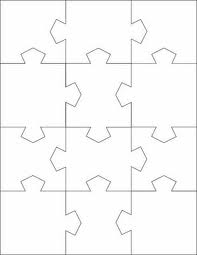
\includegraphics[height=0.1\textwidth]{rompeca} 
					\bigskip
					\pause
					
					\item El sensor de movimiento activa la particion de la imagen y la pantalla tactil es la via para mover las piezas 
					\pause
					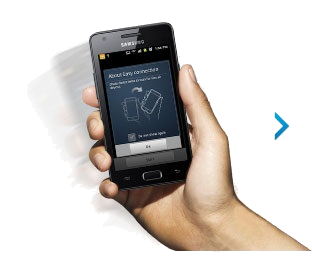
\includegraphics[width=0.1\textwidth]{shake} 
					\bigskip
					\pause
					\item La ilustracion del rompecabezas es la imagen que recibe la camara en cada fotograma
					\bigskip
					\pause
					
\includegraphics[width=0.1\textwidth]{camara1} 
					\bigskip

				\end{itemize}
			\end{frame}

		\subsection{Logros}
		
			\begin{frame}\frametitle{Resumen de logros}
				\pause \bigskip
				\begin{block}{Resumen de logros}
					\begin{columns}
						\column{.3\textwidth} \hspace{0.1cm}
						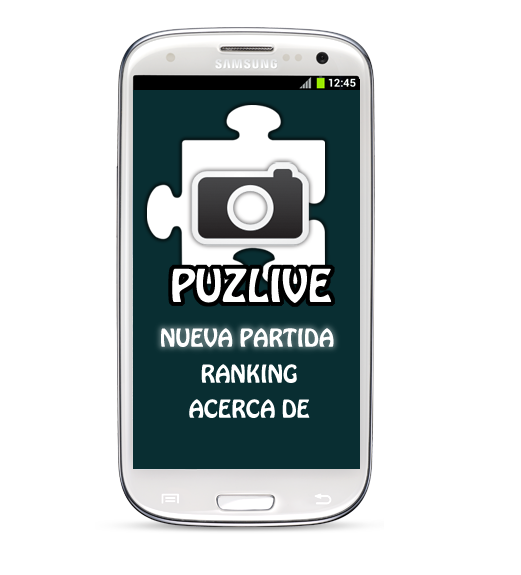
\includegraphics[width=1\textwidth]{androidpro4} 
						\column{.6\textwidth}
						Entre las caracteristicas que se penso implementar en el proyecto, los resultados fueron muy buenos con respecto
						a nuestras espectativas. Logramos establecer una interface de menus para darle al usuario una variedad de entretenimiento. 
						\\Se logro dividir la pantalla de la filmacion en celdas, mezclarlas y abilitar el SWAPING entre las celdas, 
						implementar dos tipos de juego con sus niveles de dificultad y  validar que el usuario complete el rompecabezas.
						
					\end{columns}
				\end{block}
			\end{frame}

		

	\section{Descripci\'on de los logros} 
		\subsection{Inicializar}


		\begin{frame}
			\frametitle{Icono de Aplicacion}

			\begin{block}{Icono de PuzLive}
					
				La aplicacion cuenta con su propio icono una vez instalado en el dispositivo, para inicializar la aplicaci\'on.
					
						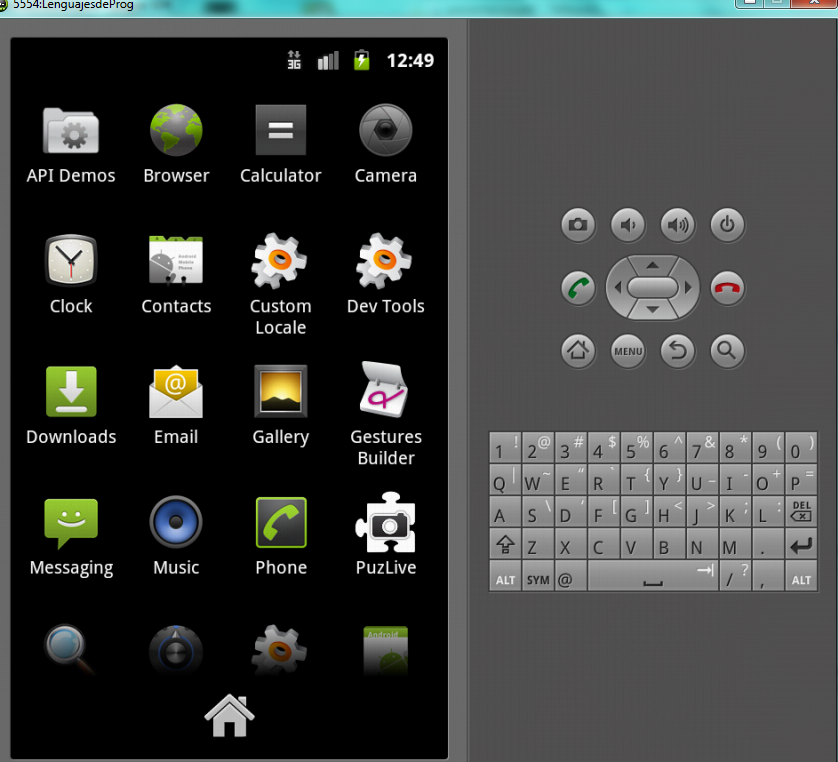
\includegraphics[width=0.5\textwidth]{outmenu} 
						\bigskip
				
				\end{block}
		\end{frame}




		\subsection{Interacci\'on}
		\begin{frame}
			\frametitle{Menu de Inicio}
				\begin{block}{Menu Inicial}
				Menu del programa, al seleccionar "Iniciar Partida" Se despliegan los diferentes tipos de juego y luego los niveles.
				\includegraphics<1>[height=5cm]{menuPrin} 
				\includegraphics<2>[height=5cm]{dosgame} 
				\includegraphics<3>[height=5cm]{niveles} 
				\end{block}
		\end{frame}

		
		
		\subsection{Rompecabezas + Video + Swaping}

		\begin{frame}
			\frametitle{Implementacion de la Camara}
				\begin{block}{Grabando y Partiendo}
					\begin{columns}
						\column{.3\textwidth} \hspace{0.1cm}
						\includegraphics<1>[width=\textwidth]{inter} 
						\includegraphics<2>[width=\textwidth]{completando} 
						\column{.5\textwidth}
						Al seleccionar uno de los niveles, la imagen se parte en distintas cantidades de celdas y se revuelven.  El swaping se logro con exito, permitiendo que 
						se pueda ordenar la imagen mezclada, tal como en un rompecabezas.
											
					\end{columns}
				\end{block}
		\end{frame}


	\subsection{Fin del Juego}
		\begin{frame}
			\frametitle{Ganador y Puntaje}
				\begin{block}{Finalizando el juego}
				Al completar la imagen real, se muestra un mensaje que valida que el usuario ha ganado y muestra el puntaje.
				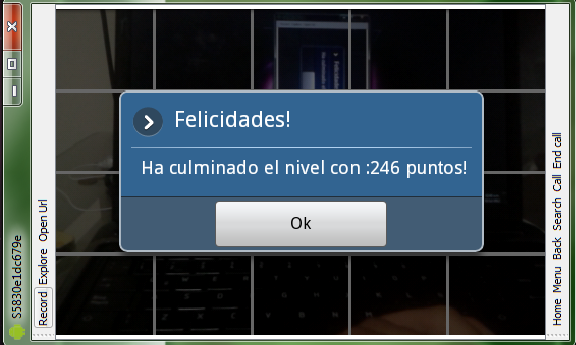
\includegraphics[height=5cm]{gano} 
				
				\end{block}
		\end{frame}

	

\end{document}